\subsubsection{La Vue}
\label{subsubsec:vue}

Chacun des deux modes de jeu possèdent une vue qui lui est propre.
Cela a été rendu possible grâce à plusieurs classes et implémentations.

Pricipalement, nous avons la classe abstraite LabyrinthView.view qui étendue par la classe \textbf{\textit{LabyrinthViewImplementation.java}}, cette classe possède comme attribut d'une instance de \\
\textbf{\textit{LabyrinthPanel.java}} qui est une classe qui étend JPanel et qui est chargée de dessiner le labyrinthe à partir de cellules crées grâce à la classe \textbf{\textit{Cell.java}} qui se basent sur les données du modèle.

Les labyrinthes ont un point de départ et un point d'arrivée que tous les joueurs doivent atteindre.

\newpage

\subsubsection*{Le mode Classique}

La vue du mode classique est gérée par la classe \textbf{\textit{LabyrinthClassicView.java}} qui est une extension de \textbf{\textit{LabyrintheViewImplementation.java}}.

\begin{figure}[!htb]
    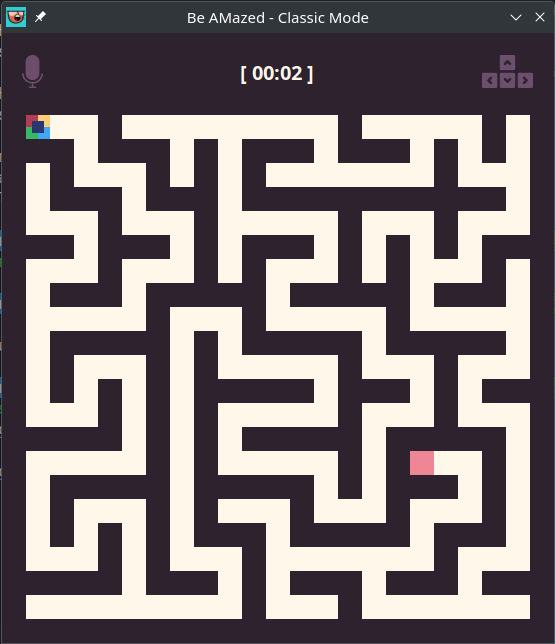
\includegraphics[scale=0.3]{ressources/Implementation/Labyrinthe/Vue/Classic/Classic.png}
    \centering
    \caption{Image du mode Classique}
\end{figure}

\subsubsection*{Le mode Blackout}

La vue du mode Blackout est gérée par la classe \textbf{\textit{LabyrinthBlackoutView.java}} qui est une extension de \textbf{\textit{LabyrintheViewImplementation.java}}.

Ce mode de jeu est un mode de jeu où les joueurs ne peuvent pas voir le labyrinthe périodiquement. Nous avons donc deux types de vues pour ce mode de jeu, une vue où le labyrinthe est visible et une vue où le labyrinthe est caché.

Les déplacements du joueur laissent derrière lui une trainée afin d'aider à se repérer dans le labyrinthe.

\begin{figure}[!htb]
    \begin{subfigure}[b]{0.3\textwidth}
        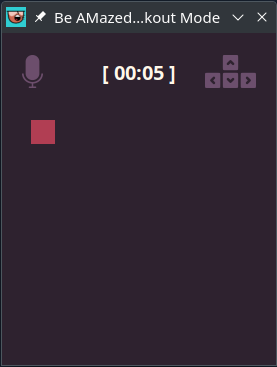
\includegraphics[width=\textwidth]{ressources/Implementation/Labyrinthe/Vue/Blackout/BlackoutDark.png}
        \caption{Labyrinthe caché}
    \end{subfigure}
    \hfill
    \begin{subfigure}[b]{0.3\textwidth}
        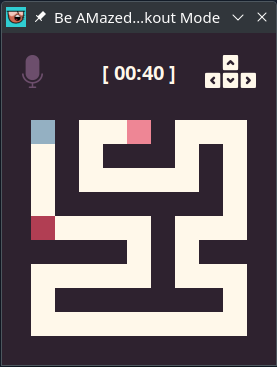
\includegraphics[width=\textwidth]{ressources/Implementation/Labyrinthe/Vue/Blackout/BlackoutLight.png}
        \caption{Labyrinthe visible}
    \end{subfigure}
    \hfill
    \begin{subfigure}[b]{0.3\textwidth}
        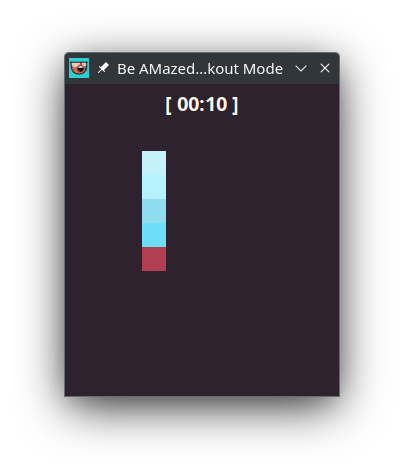
\includegraphics[width=\textwidth]{ressources/Implementation/Labyrinthe/Vue/Blackout/BlackoutDarkParticles.png}
        \caption{Labyrinthe caché et trainée}
    \end{subfigure}

    \caption{Images du mode Blackout}
\end{figure}

\subsubsection*{Les joueurs du labyrinthe}

Comme vous avez pu le voir, les joueurs dans le labyrinthe sont reprséentés par des rectangles de couleurs différentes qui changent de taille en fonction du nombre de joueurs présents sur une seule case. Nous avons choisi cette représentation car elle est simple et facile à comprendre d'un point de vu ergonomique.

\begin{figure}[!htb]
    \begin{subfigure}[b]{0.2\textwidth}
        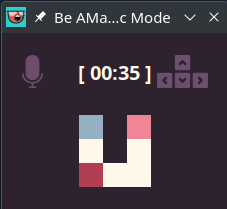
\includegraphics[width=\textwidth]{ressources/Implementation/Labyrinthe/Vue/Players/1Player.png}
        \caption{1 joueur}
    \end{subfigure}
    \hfill
    \begin{subfigure}[b]{0.2\textwidth}
        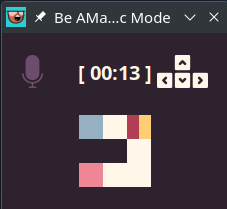
\includegraphics[width=\textwidth]{ressources/Implementation/Labyrinthe/Vue/Players/2Players.png}
        \caption{2 joueurs}
    \end{subfigure}
    \hfill
    \begin{subfigure}[b]{0.2\textwidth}
        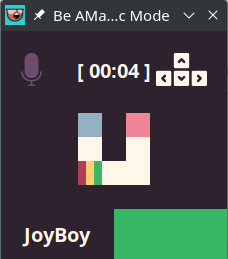
\includegraphics[width=\textwidth]{ressources/Implementation/Labyrinthe/Vue/Players/3Players.png}
        \caption{3 joueurs}
    \end{subfigure}
    \hfill
    \begin{subfigure}[b]{0.2\textwidth}
        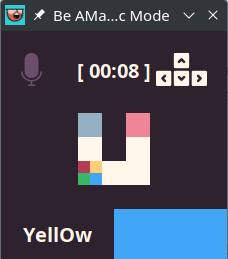
\includegraphics[width=\textwidth]{ressources/Implementation/Labyrinthe/Vue/Players/4Players.png}
        \caption{4 joueurs}
    \end{subfigure}
    \hfill
    \begin{subfigure}[b]{0.2\textwidth}
        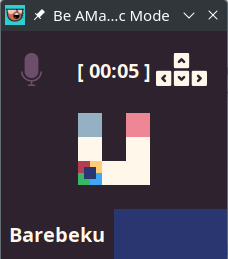
\includegraphics[width=\textwidth]{ressources/Implementation/Labyrinthe/Vue/Players/5Players.png}
        \caption{5 joueurs}
    \end{subfigure}

    \caption{Images des joueurs dans le labyrinthe}
\end{figure}

\subsubsection*{Le décompte et timer}

Le décompte et le timer sont affichés en haut au centre de chaque partie de jeu.

Le décompte affiché en rouge au début de la partie permet aux joueurs de se préparer avant le début de la partie. Une fois le décompte terminé, le timer affiché en blanc commence à compter le temps écoulé depuis le début de la partie.

\begin{figure}[!htb]
    \begin{subfigure}[b]{0.2\textwidth}
        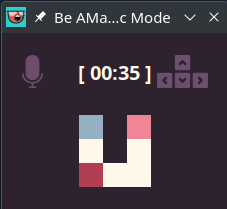
\includegraphics[width=\textwidth]{ressources/Implementation/Labyrinthe/Vue/Players/1Player.png}
        \caption{1 joueur}
    \end{subfigure}
    \hfill
    \begin{subfigure}[b]{0.2\textwidth}
        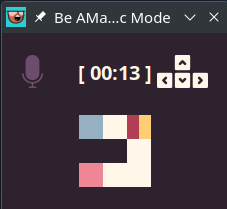
\includegraphics[width=\textwidth]{ressources/Implementation/Labyrinthe/Vue/Players/2Players.png}
        \caption{2 joueurs}
    \end{subfigure}
    \hfill
    \begin{subfigure}[b]{0.2\textwidth}
        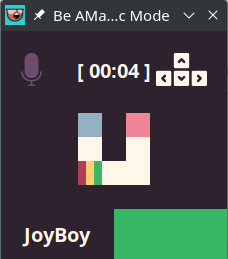
\includegraphics[width=\textwidth]{ressources/Implementation/Labyrinthe/Vue/Players/3Players.png}
        \caption{3 joueurs}
    \end{subfigure}
    \hfill
    \begin{subfigure}[b]{0.2\textwidth}
        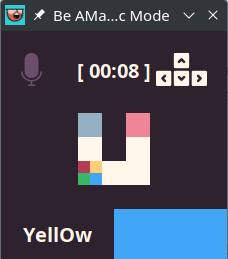
\includegraphics[width=\textwidth]{ressources/Implementation/Labyrinthe/Vue/Players/4Players.png}
        \caption{4 joueurs}
    \end{subfigure}
    \hfill
    \begin{subfigure}[b]{0.2\textwidth}
        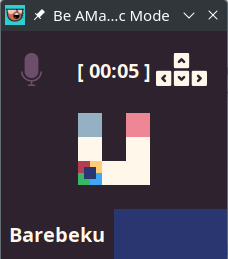
\includegraphics[width=\textwidth]{ressources/Implementation/Labyrinthe/Vue/Players/5Players.png}
        \caption{5 joueurs}
    \end{subfigure}

    \caption{Images des joueurs dans le labyrinthe}
\end{figure}

% TODO: Add images of the countdown and the timer
